\documentclass[12pt, a4paper]{article}
\usepackage[a4paper, left=2cm, right=2cm, top=3cm, bottom=3cm]{geometry}

\usepackage[english]{babel}
\usepackage[utf8]{inputenc}
\usepackage{fancyhdr}

\usepackage{enumitem}
\usepackage{amsmath}
\usepackage{mathtools}
\usepackage{listings}

\usepackage{tikz}
\usetikzlibrary{arrows.meta,shapes.multipart}

\pagestyle{fancy}
\fancyhf{}
\lhead{Tutorium 02 \\ Abgabegruppe 01}
\chead{Blatt 02 \\ DatKom}
\rhead{Andrés Montoya, 405409 \\ Til Mohr, 405959}

\begin{document}

\begin{center}\fcolorbox{red}{yellow}{\begin{minipage}{35em}
	Bei uns war ursprünglich noch ein Dritter in unserer Abgabegruppe eingeteilt. Wir haben ihn vor über einer Woche versucht per E-Mail zu erreichen, leider erfolglos.\\
	Nach Ablauf der Anmeldefrist zu den Abgabegruppen haben wir gesehen, dass diese Person leider unsere Abgabegruppe verlassen hat.\\
	Bisher konnten wir noch keinen Dritten für unsere Abgabegruppe finden.\\
	Uns wurde auch seit dem letzten Blatt keine weitere Person zugeteilt!
\end{minipage}}\end{center}



\section*{Aufgabe 2.1}


%\newpage


\section*{Aufgabe 2.2}
\begin{enumerate}[label=\alph*)]
	\item	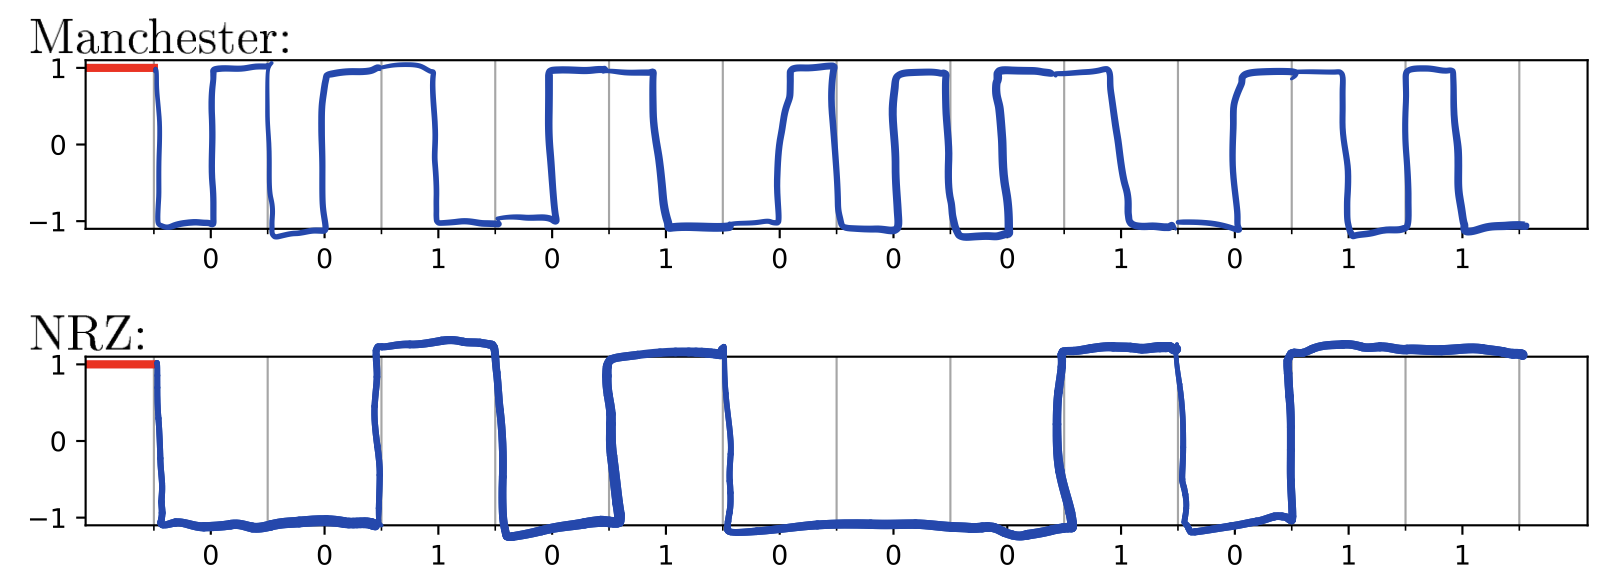
\includegraphics[scale=0.5]{2.1_a.png}
	\item	Der Manchester-Code hat eine Effizienz von $\frac{1}{2}$, da höchstes 3 Schritte notwendig sind, um ein Bit darzustellen (immer wenn 2 aufeinanderfolgende Bits gleich sind).\\
			Der NRZ-Code hat eine Effizienz von $1$, da höchstes 1 Schritt notwendig ist, um ein Bit darzustellen (immer wenn 2 aufeinanderfolgende Bits verschieden sind).\\
			
			Bei der 4B/5B-Codierung, welche NRZ verwendet, kann jede 4-Bit-Teilsequenz in höchstens 3 Schritten übertragen werden.
	\item	\begin{itemize}
				\item	In ineffizienten Codierverfahren kann man den Takt einbauen $\rightarrow$ Selbsttaktung $\rightarrow$ Falsche Synchronisation leicht zu erkennen
				\item	Redundanz
			\end{itemize}
	\item	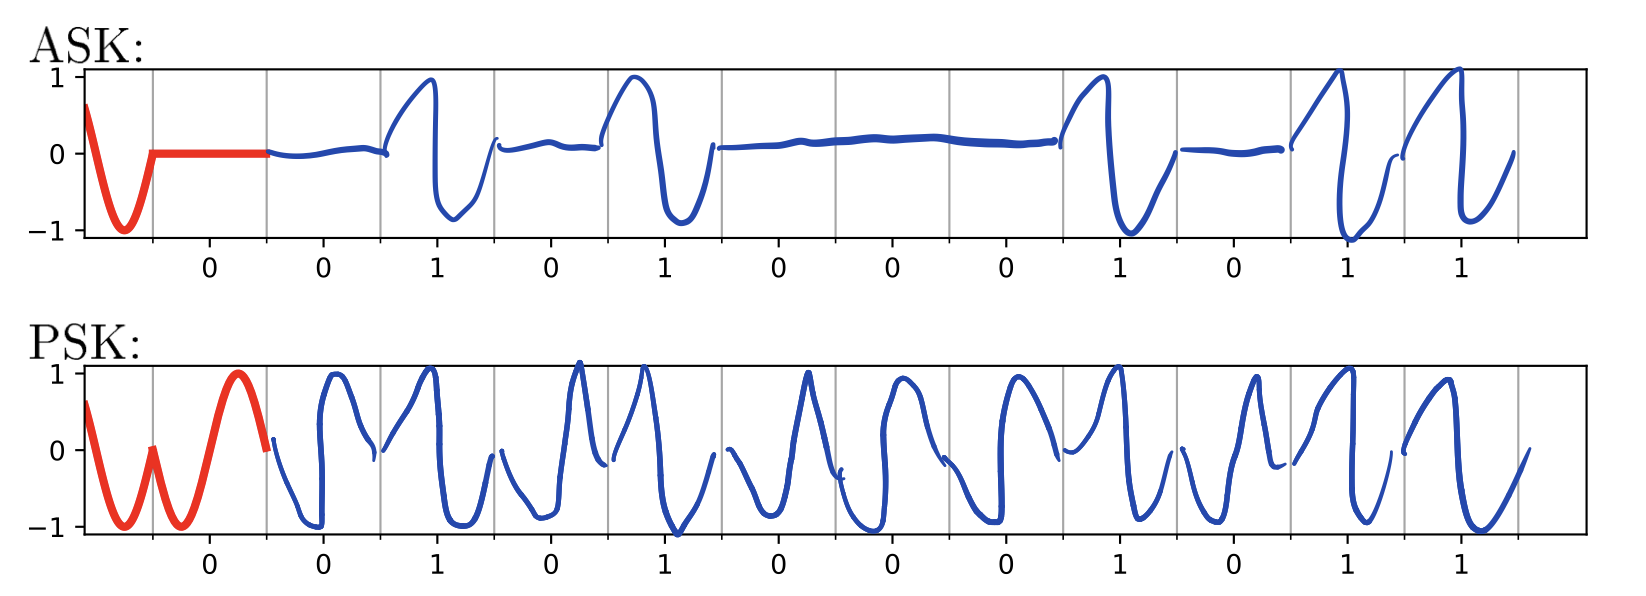
\includegraphics[scale=0.5]{2.1_d.png}
\end{enumerate}


\newpage


\section*{Aufgabe 2.3}
\begin{enumerate}[label=\alph*)]
	\item	$$l \coloneqq \frac{100 km}{299792458 \frac{m}{s}} = 333.564095198 \mu s$$
	\item	\textit{"die Bestätigung des 1. Bits"} ist etwas undeutlich formuliert, da normalerweise keine Bestätigungen auf der Bitübertragungsschicht stattfinden, und dies daher protokollabhängig ist. Wir gehen davon aus, dass mit dieser Teilaufgabe die Kapazität in beide Richtungen gefragt ist.
			$$c \coloneqq 100 \frac{Gbit}{s} \cdot l \cdot 2 = 66.7128190396 \frac{Mbit}{s}$$
	\item	\begin{enumerate}[label=\roman*)]
				\item	$$60 dB = 10 \cdot \text{ld}(S/N) \Leftrightarrow S/N = 10^{\frac{60}{10}} = 10^6$$
						Also ist das Eingabesignal $10^6$ mal stärker als das Ausgabesignal. Da das Ausgabesignal einen Mindestleistungspegel von $-10 dBm$ verlangt, muss das Eingabesignal einen Mindestleistungspegel von $10^6 \cdot -10 dBm$ haben.
						$$10^6 \cdot -10 dBm = 10 \cdot \text{ld}(\frac{P}{1 mW}) \Leftrightarrow P = 1 mW \cdot 10^{\frac{10^6 \cdot -10 dBm}{10}} = 1 mW \cdot 10^{-10^6 dBm} \rightarrow 0$$
						
						\textbf{??? Hier ist ein Fehler drinnen!}
				\item	
			\end{enumerate}
\end{enumerate}


\newpage


\section*{Aufgabe 2.3}
\begin{enumerate}[label=\alph*)]
	\item	Wir haben $64$ Signalstufen, die wir also mit $\text{lb}(64) = 8$ Bit jeweils darstellen können. Nach Nyquist gilt:
			$$180 \frac{MBit}{s} = 2 \cdot B \cdot 8 Bit \Leftrightarrow B = 11250 Hz$$
	\item	$$SNR_{db} = 10 \cdot \text{ld}(S/N) \Leftrightarrow S/N = 10^{\frac{SNR_{db}}{10}} \Rightarrow S/N = 10^{\frac{50 dB}{10}} = 10^5$$
			Nach Shannon gilt:
			$$D = B \cdot \text{ld}(1 + S/N) \Rightarrow D = 11250 Hz \cdot \text{ld}(1 + 10^5) \approx 56250 \frac{Bit}{s}$$
			Da $D < R$ ist die maximale Datenrate gleich $D$.
	\item	
\end{enumerate}


\end{document}